%------------------------------------------------------------------------------
% Template file for the submission of papers to IUCr journals in LaTeX2e
% using the iucr document class
% Copyright 1999-2013 International Union of Crystallography
% Version 1.6 (28 March 2013)
%------------------------------------------------------------------------------

\documentclass[preprint]{iucr}              % DO NOT DELETE THIS LINE

     %-------------------------------------------------------------------------
     % Information about journal to which submitted
     %-------------------------------------------------------------------------
     \journalcode{J}              % Indicate the journal to which submitted
                                  %   A - Acta Crystallographica Section A
                                  %   B - Acta Crystallographica Section B
                                  %   C - Acta Crystallographica Section C
                                  %   D - Acta Crystallographica Section D
                                  %   E - Acta Crystallographica Section E
                                  %   F - Acta Crystallographica Section F
                                  %   J - Journal of Applied Crystallography
                                  %   M - IUCrJ
                                  %   S - Journal of Synchrotron Radiation
\usepackage{graphicx}
\usepackage[T1]{fontenc}
\usepackage[utf8]{inputenc}
\usepackage{amsmath}

\begin{document}                  % DO NOT DELETE THIS LINE

     %-------------------------------------------------------------------------
     % The introductory (header) part of the paper
     %-------------------------------------------------------------------------

     % The title of the paper. Use \shorttitle to indicate an abbreviated title
     % for use in running heads (you will need to uncomment it).

\title{Application of signal separation to diffraction image compression and serial crystallography}
%\shorttitle{Short Title}

     % Authors' names and addresses. Use \cauthor for the main (contact) author.
     % Use \author for all other authors. Use \aff for authors' affiliations.
     % Use lower-case letters in square brackets to link authors to their
     % affiliations; if there is only one affiliation address, remove the [a].

\cauthor[a]{Jérôme}{Kieffer}{jerome.kieffer@esrf.fr}{}
\author[a]{Nicolas}{Coquelle}
\author[a]{Samuel}{Debionne}
\author[b]{Shibom}{Basu}
\author[a]{Alejandro}{Homs}
\author[a]{Gianluca}{Santoni}
\author[a]{Götz}{Andrew}
\author[a]{Daniele}{De Sanctis}

\aff[a]{European Synchrotron Radiation Facility;71, avenue des Martyrs;CS 40220;38043 Grenoble Cedex 9 \country{France}}
\aff[b]{EMBL Grenoble; 71 avenue des Martyrs; CS 90181; 38042 Grenoble Cedex 9; \country{France}}

     % Use \shortauthor to indicate an abbreviated author list for use in
     % running heads (you will need to uncomment it).

%\shortauthor{Soape, Author and Doe}

     % Use \vita if required to give biographical details (for authors of
     % invited review papers only). Uncomment it.

%\vita{Author's biography}

     % Keywords (required for Journal of Synchrotron Radiation only)
     % Use the \keyword macro for each word or phrase, e.g. 
     % \keyword{X-ray diffraction}\keyword{muscle}

%\keyword{keyword}

     % PDB and NDB reference codes for structures referenced in the article and
     % deposited with the Protein Data Bank and Nucleic Acids Database (Acta
     % Crystallographica Section D). Repeat for each separate structure e.g
     % \PDBref[dethiobiotin synthetase]{1byi} \NDBref[d(G$_4$CGC$_4$)]{ad0002}

%\PDBref[optional name]{refcode}
%\NDBref[optional name]{refcode}

\maketitle                        % DO NOT DELETE THIS LINE

\begin{synopsis}
Precise background assessment and application to single crystal image compression and serial crystallography data pre-processing. 
\end{synopsis}

\begin{abstract}

This contribution is about real-time analysis of diffraction images acquired at high frame-rate (1 kHz) and its applications to macro-molecular serial crystallography.
A new signal separation algorithm will be presented, able to distinguish amorphous (or powder diffraction) component from the signal originating from larger (single) crystals.
It relies on the ability to work efficiently in azimuthal space and derives from the work performed on pyFAI, the fast azimuthal integration library.
Two applications are built upon this separation algorithm: a lossy compression algorithm and a peak-picking algorithm.
Their performances will be assessed and compared to state of the art reference implementations using XDS and CrystFEL.


\end{abstract}


     %-------------------------------------------------------------------------
     % The main body of the paper
     %-------------------------------------------------------------------------
     % Now enter the text of the document in multiple \section's, \subsection's
     % and \subsubsection's as required.

\section{Introduction}
The main limitation of rotational crystallography, where a complete dataset is collected from a single crystal rotated around one (or several) axis, is radiation damage resulting from the exposure to the  beam.
In macro-molecular crystallography (MX), several crystals are often needed to collect a complete dataset.
Serial crystallography overcomes radiation damage by exposing each crystal a single time, thus, thousands of them are exposed in a serial way to collect a complete dataset.
%Crystals are exposed in a serial way to the beam with random orientation, giving making the data-reduction of

\subsection{Serial crystallography using synchrotron sources (SSX)}
%not sure we need subsections here
%Serial crystallography is a relatively new technique in structural biology. 
%It is composed of several techniques where multiple crystals (hundreds or thousands) are exposed in a serial %way to the X-ray beam to collect a complete dataset. 
%This is in contrast with traditional rotational crystallography, where a complete dataset is collected from a single crystal rotated around one (or several) axis. 
%The serial approach is particularly useful to try to overcome the limitations of radiation damage in %rotational crystallography, particularly in very small crystals.

The technique was first developed for X-ray free electron lasers (\textsc{xfel}) \cite{Chapman2011, structure_sx} and then adapted to be performed at synchrotron light sources \cite{ssx, ssx_desy, ssx_id13, ssx_diamond}.
However, macromolecular crystallography beam-lines (MX) have been extremely specialized towards rotational data-collection and are thus not well adapted to SSX.
The high flux needed to collect all diffraction signal from a single crystal within a single exposure makes  the SSX technique a good candidate to benefit from the 4\textsuperscript{th} generation synchrotron sources, such as the new ESRF-EBS update \cite{EBS}.
The synchrotron serial crystallography beamline (ID29 at the ESRF) has been built to have a dedicated environment to perform SSX experiments with a high flux (thanks to multi-layer optics), a high-speed chopper (to separate photon bunches), several sample delivery methods and a fast detector.

\subsection{Jungfrau-4M detector}
Macro-molecular crystallography has enormously progressed in the last decades with to the introduction of photon-counting detectors \cite{pilatus}. 
With their absence of read-out noise and their fast speed, the main limitation of photon-counting detectors is the achievable count-rate, i.e. how fast the electronic of a pixel is able to count arriving photons.
% difference bewteen pixel counting vs integrating, in speed ...
Unlike photon-counting detectors such as the Eiger detector \cite{Eiger}, the Jungfrau detector \cite{jungfrau2016} is an integrating detector, thus, it is not limited by the count rate, even under the very intense flux expected when recording Bragg-peaks.
To cope with this photons density, every single pixel implements an automatic gain switching mechanism (3 levels) which offers a precision of the order of one third of a keV on the higher gain mode, a precision of the order of one photon in the intermediate level and the ability to cope with thousands of photons in the lower gain mode, every millisecond.
Since the Jungfrau detector is an integrating detector, dark current and flat-field correction have to be applied: every pixel has three, so called, pedestals and three gain values (one for each gain level). 
However, this large number of parameters per pixel combined with the gain-compression makes the pre-processing of raw signal challenging: the signal from a single pixel, initially stored on 16 bits of data, needs to be represented using 32 bits (as floating point or integer value), doubling the required bandwidth and the storage size \cite{jungfrau_PSI}.
The ID29 beam-line features a Jungfrau-4M detector, operating at 1kHz, pace imposed by the chopper and synchronized with the photon bunches from the ESRF.
At nominal speed, this beam-line is expected to produce 20 GBytes of pre-processed data per second, making the data analysis and storage extremely challenging.

\subsection{Requirements for online data processing}

Serial crystallography is one of the techniques where online data processing is likely to have most impact:
millions of images are to be collected but too fast to be saved. 
On the other hand only about 10\% of them will contain diffraction signal and out of them, about half can be indexed and integrated and will actually be used to solve the crystal structure.
Thus efficient processing of raw images is essential for SSX, with 4 levels of increasing complexity:
\begin{itemize}
    \item image reconstruction with pedestal correction
    \item \textit{veto-}algorithm: be able to sieve-out images with poor signal
    \item save only pixels with diffraction signal
    \item precise location of peak position with indexation
    \item real-time integration of diffraction peaks
\end{itemize}.

The first level has been described in \citeasnoun{lima2}.
This document will focus on subsequent steps: the third point is addressed in section 2 and the fourth in section 3, leaving real-time integration as a challenge for the future.
%The second step is to collect only pixel values corresponding to diffraction signal.
%or even an algorithm able to point.

% 1e6 images, 100k hits, 10k indexed and integrated images
% for each of the individual frame low partiallity need 10k frames/crystall to get a complete dataset with enough redundancy



%Multiple challenges are present, in particular partiality and low completeness of data collected for each individual crystal.
%For this reason, careful and precise location of Bragg peaks is essential.



%The document is sub-divided like 
%Section 2 presents an efficient way to separate Bragg-peaks from background, this technique is used in section 3 to compress MX data using sparsification of data. 
%The data 

\section{Algorithm for the separation of the amorphous background from the Bragg peaks}
\subsection{Background scattering}
%be careful & be precise ...
The simplest implementation of Bragg peaks separation is to assume that the background signal originates from scattering of amorphous material (or from an isotropic powder), giving an isotropic signal that ideally presents only smooth variations.
For this, the raw signal has to be corrected for dark noise and for any systematic anisotropic effects such as polarization corrections.
Unlike X-FEL, synchrotron X-ray beam is better characterized in energy and shows little bunch-to-bunch variability.
All anisotropic correction can be easily modeled and taken into account.

%the first thing is to get it working, the second is to make it fast ... coming from another field of science.
The initial implementation of signal separation in pyFAI \cite{pdj2013} was relying on a 2D polar transform followed by a median filter in the azimuthal dimension to calculate the amorphous scattering curve.
Although this method has been successfully used for large dataset analysis \cite{brocades}, it presents four major drawbacks:
\begin{itemize}
\item The 2D averaging mixes the signal originating from several pixels and blurs the signal. 
\item Pixel-splitting is needed to leverage the Moiré effect in the 2D averaging, but this further increases the blurring. 
\item The 1D curve obtained after the application of the median filter shows sharp jumps from one azimuthal bin to its neighbour.
\item The median filter is computationally heavy since it is required to sort out every azimuthal bin.
\end{itemize}

The following sections present an efficient way of performing the azimuthal averaging (including the associated uncertainty propagation),  its application to the statistical analysis in polar space and the extraction of background from a diffraction image. 

\subsection{Efficient azimuthal averaging and uncertainties evaluation}

\subsubsection{Pre-processing:}
The first step of the analysis consists in applying a pixel-wise correction for dark current and several normalization corrections \cite{pyfai_2020}:
\begin{equation}
\label{norm}
I_{cor} = \frac{signal}{norm}  = \frac{I_{raw} - I_{dark}}{F \cdot
\Omega \cdot P \cdot A \cdot I_0} 
\end{equation}
In  equation \ref{norm}, the numerator (referred as \textit{signal} hereafter) is the subtraction of the dark current $I_{dark}$ from the the detector's raw signal $I_{raw}$.
The denominator (hereafter \textit{norm}) is a normalization factor composed of the product of  $F$:  a factor accounting for the flat-field correction, $\Omega$: the solid angle subtended by a given pixel, $P$: the polarisation correction term and $A$: the detector's apparent efficiency due to the incidence angle of the photon on the detector plane. 
For integrating detectors, photons with high energy see longer sensor path with larger incidence angles compared to the normal thickness, thus they have a higher detection probability.
Intensity is also normalized by the incoming flux $I_0$, but since it is independent from the pixel position this correction can be applied when convenient.

\subsubsection{Azimuthal averaging:} 

Historically, the azimuthal averaging was implemented using histograms. 
Since the geometry of the experimental setup is fixed during the acquisition, a look-up table listing all pixels contributing to each  azimuthal-bin can be built and used to speed-up calculations \cite{pyFAI_gpu}.
The azimuthal transformation being a linear transformation, it can be implemented as a matrix multiplication, with a sparse-matrix representing the transformation and a dense vector that is simply the flattened view of the diffraction image. 
The compressed sparse row (CSR) matrix representation is preferred for its efficiency in performing dot products with dense vectors \cite{SpMV}.
The coefficients $c_{i,r}$ of the matrix are the fraction of area of a pixel $i$ falling into the radial bin $r$.
In the case where pixel splitting is deactivated these coefficients  ($c_{i,r}$) are always one (and zero elsewhere) since each pixel contributes to a single bin.
The sparse matrix multiplication can be used to sum efficiently values for all pixels belonging to the same bin.
The summed signal divided by the summed normalization provides the weight-averaged intensity over all pixels falling in the bin at the distance $r$ from the center, as formalized in equation \ref{avg}: 
\begin{equation}
\label{avg}
<I>_{r} = \frac{\sum\limits_{i \in bin_r} c_{i,r} \cdot signal_i}
                        {\sum\limits_{i \in bin_r} c_{i,r} \cdot norm_i} 
\end{equation}  

\subsubsection{Uncertainty evaluation from Poisson law:}
Photon counting detectors, such as Eiger detectors, suffer from hardly any error beside the counting uncertainty which is often referred to as Poisson statistics.
This statistical law states is described by a single parameter $\lambda$ which is related to the mean $\mu$ and standard deviation $\sigma$ from normal distribution by: $\lambda=\mu=\sigma^2$.
Other sources of noise, like the dark current noise in the case of an integrating detector,  superimpose quadratically on the Poisson noise for integrating detectors, as presented in equation \ref{poisson}:     
\begin{equation}
\label{poisson}
var_I = (\sigma_I)^{2} = <I_{raw}> + (\sigma_{dark})^{2}  
\end{equation}

During the azimuthal integration, the coefficient of the sparse matrix needs to be squared at the numerator when propagating the variance (equation \ref{varianceP}) to have uncertainties $\sigma$ proportional to the fraction of the pixel considered.
\begin{equation}
\label{varianceP}
(\sigma_{r}(I))^2 = \frac{\sum\limits_{i \in bin_r} c_{i,r}^2 \cdot \sigma_i^2}
                  {\sum\limits_{i \in bin_r} c_{i,r} \cdot norm_i} 
\end{equation}
One should distinguish the \textit{uncertainty of the mean} (sometimes referred to as the standard error of the mean or $sem$), 
which describes the precision with which the mean is known (and described in \citeasnoun{pyfai_2020}),
from the \textit{uncertainty of the pixel value} (often referred to as standard deviation, $std$) which describes the uncertainty with which the pixel value is known. 
Those two value differ only by the square root of the number of measurements in the case of an arithmetic mean: $sem = std/\sqrt{N}$ with $N$ being the number of pixel contributing to the bin.
When considering the weighted average, the previous formula becomes:
\begin{equation}
\label{sem}
sem_r = std_r \frac{\sqrt{\sum\limits_{i \in bin_r} c_{i,r}^2 \cdot norm_i^2}}{\sum\limits_{i \in bin_r} c_{i,r} \cdot norm_i}
\end{equation}
Thus, the more data points are collected, the more precisely the mean value is known but the uncertainty for a given point remains the same.
Since this document focuses on the uncertainties of pixel values, the \textit{standard deviation} will systematically be used in this document.  

\subsubsection{Uncertainty evaluation from the variance in a bin:}

Unlike photon counting detectors, most detectors are not following the Poisson law and therefore the establishment of a formula $\sigma^2 = f(I)$ is not simple, if possible at all. 
In the case of the Jungfrau detector, this integrating detector has a complex gain switching mechanism \cite{jungfrau_PSI} which makes this equation complicated.
A generic approach is proposed here to measure the variance in every single azimuthal bin.

When considering the diffraction of an isotropic compound (liquid, amorphous or perfect powder), all pixels falling into the same radial bin should see the same flux of photons and the deviation to their intensities can be used to estimate the uncertainty. 
This approach is of course limited when considering Bragg-peaks, but it provides an upper bound for the uncertainty.
Variance (thus standard deviation) are usually obtained in a two steps procedure: one pass to calculate the average value (equation \ref{avg}) and a second to calculate the deviation to the average (equation \ref{varA}). 
This double pass approach can be implemented using sparse matrix multiplication. 
It requires twice the access to each pixel value, and extra storage space, but it is numerically robust (i.e. not prone to numerical error accumulation).
\begin{equation}
\label{varA}
    (\sigma_{r}(I))^2 = \frac {\sum\limits_{i \in bin_r} c_{i,r} \cdot norm_i \cdot (\frac{signal_i}{norm_i}-<I>_r)^2}
                              {\sum\limits_{i \in bin_r} c_{i,r} \cdot norm_i}
\end{equation}
and:
\begin{equation}
\label{varB}
(\sigma_{r}(<I>))^2 = \frac{\sum\limits_{i \in bin_r} c_{i,r}^2 \cdot norm_i^2 \cdot (\frac{signal_i}{norm_i}-<I>_r)^2}
                         {(\sum\limits_{i \in bin_r} c_{i,r} \cdot norm_i)^2}  
\end{equation}


Single pass implementations of variance calculation are faster since they access pixels only once and offer the ability to perform parallel reductions \cite{Blelloch}, i.e. work with blocks of pixels.
\citeasnoun{variance2018} present a complete review on the topic, which introduces a formalism adapted here for crystallography.
For example the weight for a pixel is $\omega_i = c_i \cdot norm_i$.
If $P$ is a partition of the ensemble of pixels falling into a given azimuthal bin, let $\Omega_{P}$, $V_{P}$ and $VV_{P}$  
be the sum of weights (Eq \ref{omega}), the weighted sum of $V$ (Eq. \ref{Vp}) and the weighted sum of deviation squared (Eq \ref{VVp}) over the partition $P$: 
\begin{equation}
\label{omega}
\Omega_{P} = \sum\limits_{i \in P} \omega_i = \sum\limits_{i \in P} c_i \cdot norm_i 
\end{equation}
\begin{equation}
\label{Vp}
V_{P} = \sum\limits_{i \in P} \omega_i \cdot v_i =  \sum\limits_{i \in P} c_i \cdot signal_i
\end{equation}
\begin{equation}
\label{VVp}
VV_{p} = \sum\limits_{i \in P} \omega_i \cdot (v_i - V_{P}/\Omega_{P})^2 
\end{equation}

The average and the variance are then expressed as:
\begin{equation}
\label{eq11}
<I>_P = \frac{V_{P}}{\Omega_{P}} =  \frac{\sum\limits_{i \in P} c_i \cdot signal_i}
                        {\sum\limits_{i \in P} c_i \cdot norm_i} 
\end{equation}

\begin{equation}
\label{eq12}
(\sigma_P(I))^2 = \frac{VV_{P}}{\Omega_{P}}
\end{equation}

In this formalism, equations \ref{avg} and \ref{eq11} on one side and equations \ref{varA} and \ref{eq12} are actually the same.
In their review, \citeasnoun{variance2018} present the way to perform the union of two sub-partitions $A$ and $B$ of a larger ensemble which opens the doors to parallel reductions, which are especially efficient when implemented on GPU:
\begin{equation}
\label{13}
\Omega_{A \cup B} =  \Omega_{A} + \Omega_{B} 
\end{equation}

\begin{equation}
\label{14}
V_{A \cup B} =  V_{A} + V_{B} 
\end{equation}
  
\begin{equation}
\label{15}
VV_{A \cup B} =  VV_{A} + VV_{B} +  \frac{(\Omega_{A} \cdot V_{B} - \Omega_{B}\cdot V_{A})^2}{V_{A \cup B} \cdot  V_{A} \cdot V_{B}}
\end{equation}
While equations \ref{13} and \ref{14} are trivial, equation \ref{15} has a term of cross-contribution.
A numerical stability issue can arise from it when $V_A$ or $V_B$ is very small and this issue is addressed by using double-precision arithmetic when implemented on CPU and double-word arithmetic when running on GPU \cite{double_word}.

\subsection{Histogram intensity }

The figure \ref{fig1}a presents the diffraction from a single crystal of insulin with a Pilatus 6M detector and several curves obtained from azimuthal integration of those data: 
figure \ref{fig1}b is the azimuthally integrated signal (blue curve) where Bragg peaks are seen as spikes on top of a smooth background.
The plot \ref{fig1}c presents the uncertainties measured according to the Poisson law (orange curve, valid since Pilatus are photon counting detectors) 
or the deviation in the ring (blue curve). 
The later presents much larger values since Bragg peaks contribute a lot to the deviation despite they represent few pixels: this highlights the sensitivity of the mean/std to outliers.
In the plot \ref{fig1}d are presented histogram of pixel intensity for pixels laying at 87mm and 160mm from the beam center. 
Each of those histograms is composed of a bell-shaped distribution, centered on the average value with negative outliers tagged with the pixel value -1 (this is specific to the Pilatus detector), and few positive outliers which are usually Bragg peaks.   
Those histograms in figure \ref{fig1}d have been fitted with a Gaussian curve and both the center ($\mu$) and the width ($\sigma$) of the curve match 
roughly with the average (in \ref{fig1}b) and uncertainties (in \ref{fig1}c).  
\begin{figure}
\label{fig1}
\begin{center}
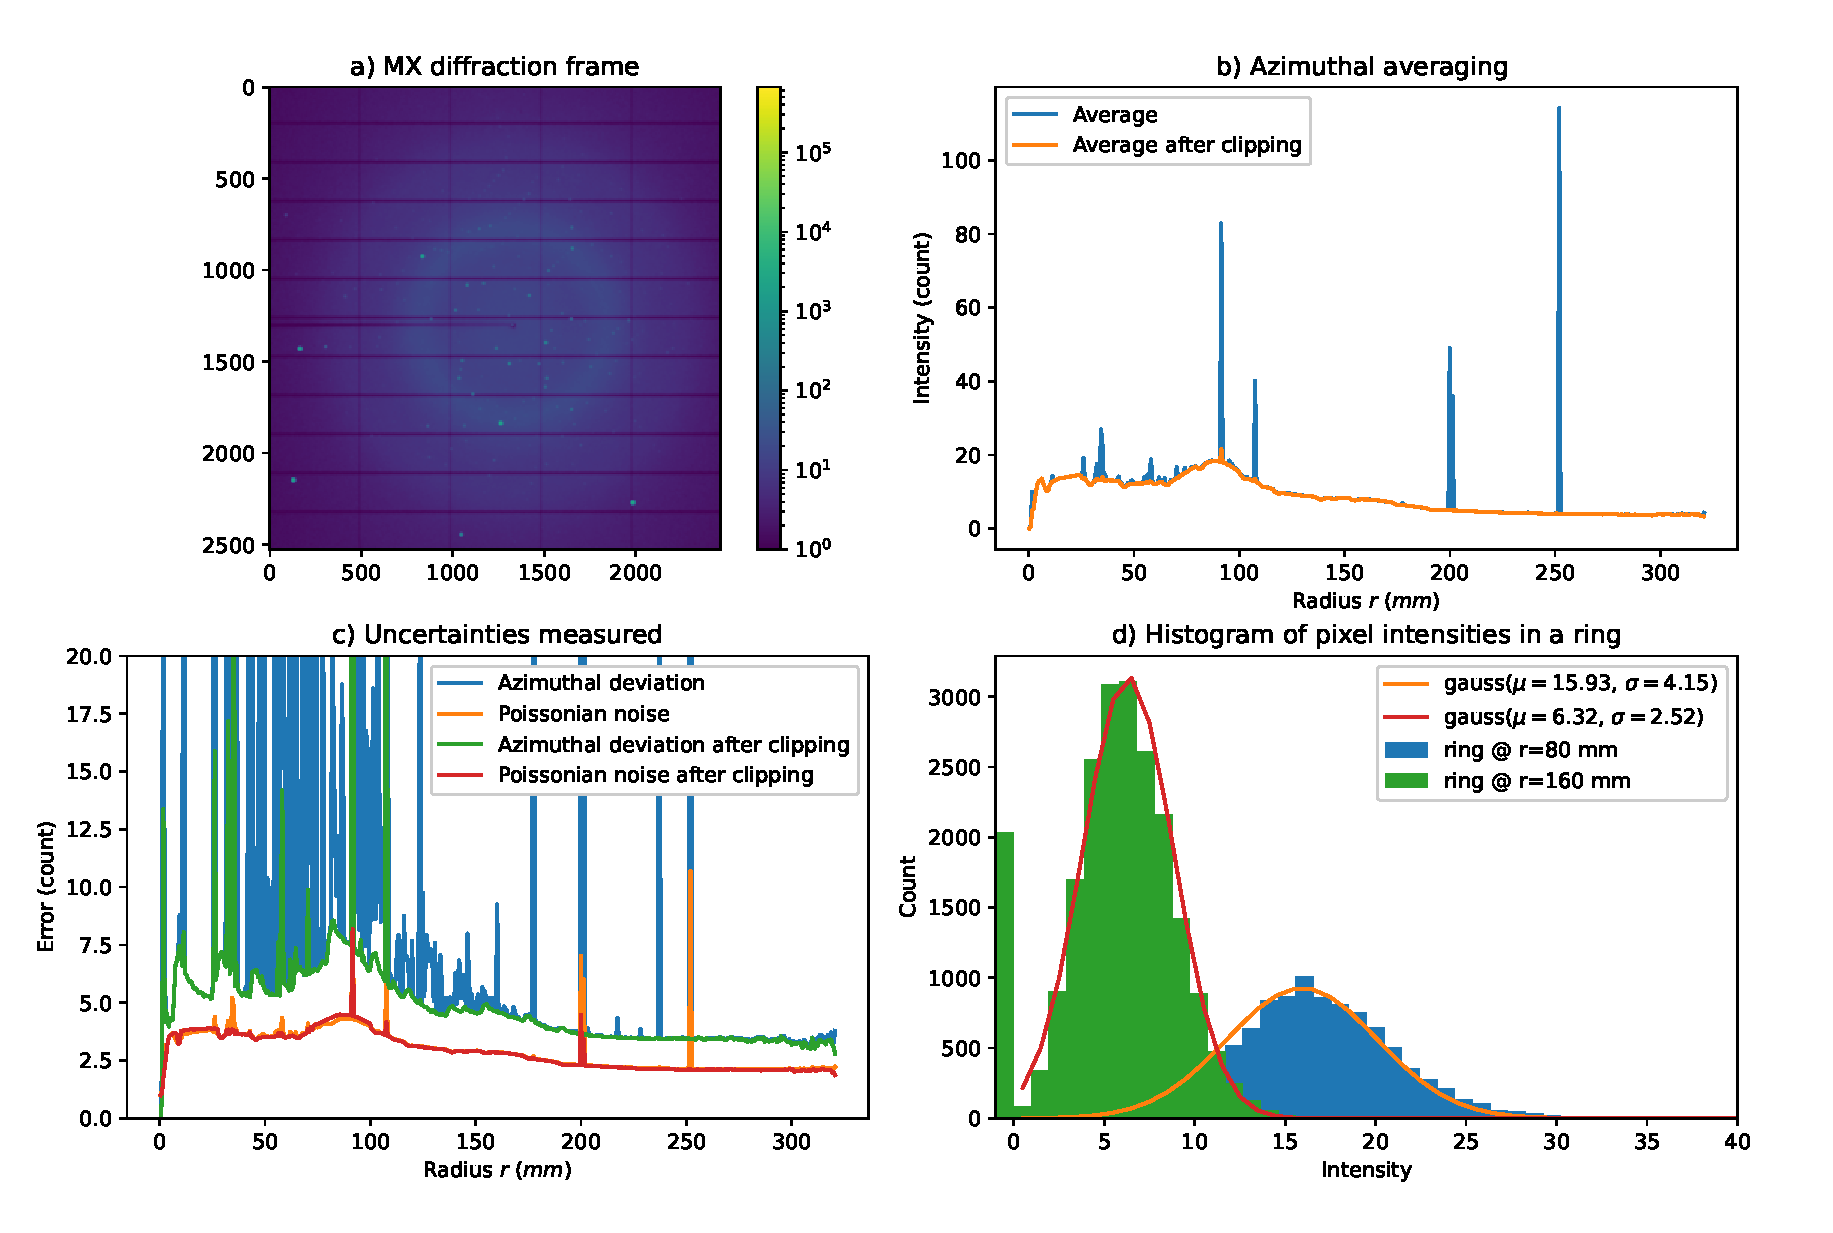
\includegraphics[width=14cm]{fig1}
\caption{Single crystal diffraction frame obtained from insulin with a Pilatus 6M (a) with the azimuthally averaged signal (b), 
before and after clipping data. Uncertainties are presented in (c) when calculated assuming a Poissonian error model (orange, red) or when measuring the deviation within all pixels in a ring (green, blue).
Subplot (d) presents the histogram of intensities for two rings at r=87mm and r=160mm from beam center with the distribution fitted as Gaussian curves: $g(x)\propto exp(-\frac{(x-\mu)^2}{2\sigma^2})$.}
\end{center}
\end{figure}

The core idea of the algorithm for background extraction is to model the distribution of background pixels. Unlike Bayesian statistics \cite{Sivia2006} where the cost function is usually tuned to weight less outlier, here, those outliers are simply flagged and discarded.
Positive outliers can reasonably be assigned to Bragg peaks and negative outliers to shadows or defective pixels. 
The distribution is recalculated  after discarding pixels for which intensity differ from the average value by more than $n$ times the standard deviation (Eq. \ref{clip}), where $n$ is called the Signal over Noise Ratio (SNR).
This clipping re-centers the distribution of remaining pixels since the mean is sensitive to outlier values:
\begin{equation}
\label{clip}
|I - <I>| > n \cdot \sigma(I)
\end{equation}
The orange plot in figure \ref{fig1}b presents the average after having discarded those outliers, and the orange and green curve of figure \ref{fig1}c are the uncertainties calculated after this clipping. 
After clipping, the average and uncertainties curves have lost most of their spikes, which means that most Bragg peaks and shadowed pixel have been discarded.
 
\subsection{Sigma-clipping}
The \textit{sigma-clipping} algorithm consists in applying the outlier rejection, previously described, several times.
If the initial distribution was mono-modal, this algorithm enforces gradually the background pixels towards a normal distribution.
If the initial distribution was more complicated (typically multi-modal), few pixels are likely to be rejected  due to large standard-deviation.
This algorithm takes two parameters: the number of iterations and the rejection cut-off (SNR).
%I merged number of iterations and sigma clipping  as closely connected.
Despite the execution time is proportional to the number of iteration of sigma-clipping, iterations should continue until no more outliers are found, so that the background data can be treated assuming a normal distribution. 
Since the loop exits as soon as no more outliers were discarded at the clipping step, having an arbitrary large number of iteration is not really an issue for the execution time and the number of actual iteration is usually few (3 is commonly observed).       

\subsubsection{Limits of the Poissonian approach:}
The evaluation of uncertainties based on the variance over a radial shell has been developed after numerical artifacts were discovered when performing sigma-clipping with a Poissonian approach. Some azimuthal bins where exhibiting no pixel contribution at all and thus appeared without any mean nor uncertainties, jeopardizing the complete background extraction algorithm. 
This artifact was directly linked to the usage of Poisson statistics and can be demonstrated with a simple distribution of 2 pixels, having values 1 and 199. 
The mean of this distribution is 100 and the standard deviation is also close to 100 while the uncertainty derived from a Poissonian law would  be close to 10 (i.e. $\sqrt{100}$). 
With the azimuthal error model, both pixels are a $1\sigma$ from the mean while with the Poissonian error-model, pixels are at $10 \sigma$.  
This explains why bins featuring strong Bragg-peaks on top low background got completely emptied from all their contributing pixels when sigma-clipping was performed, assuming Poissonian noise.

\subsubsection{Clipping threshold}
can be automatically calculated based on a variation on Chauvenet's criterion \cite{chauvenet} where one would accept to discard only a single pixel in a ring with a signal already following a normal law. 
Thus, the threshold value is adapted to the $size$ of the distribution, i.e. the number of pixels in each ring (Eq. \ref{chauvenet}), which can reach several thousands and shrinks with iterations.
Typically the numerical value for this cut-off varies from 2 to 4.   
\begin{equation}
\label{chauvenet}
SNR_{chauv.} =  \sqrt{2 log(\frac{size}{\sqrt{2 \pi}})}
\end{equation}

The worse case scenario for sigma-clipping is when the initial distribution is very far from being normal, for example bimodal distribution as seen in previous paragraph.
Another challenging situation occurs close to the detector corners where the background signal is low and the size of the distibution is decreasing. 
If the ensemble counts 100 (respectively 1000) pixels, the automatic clipping parameter evaluates to $SNR_{chauv.} = 2.7$ (respectively $SNR_{chauv.} = 3.5$).
Let's assume the detector has a Poissonian behaviour and the signal is very low: $\lambda = \mu = \sigma^2 = 1$. 
Any pixels with intensity 4 (respectively 5) or higher are discarded. 
Pixel values are integers here since the detector is counting events (or a consequence of the Poisson law).
% could be interesting to show Threshold vs cycle for the example above (if relecant)

\section{Application to single crystal diffraction image compression}
%I explicit here MAcromolecular as we are talking about id29. Remove is superfluous.
Diffraction images from a single macro-molecular crystal exhibit usually an isotropic background on top of which Bragg peaks appear.
The sigma-clipping algorithm can be used to select the background level and more importantly the associated uncertainty.

This lossy compression algorithm consists in picking (and storing) pixels which intensity is above the average background value ($\mu$) plus $n$ standard deviation ($\sigma$). 
This cut-off value $n$ (also called $SNR_{pick}$) controls the amount of data to store and provides also a hint for the compression ratio achievable, assuming a normal distribution has been enforced at the sigma-clipping stage: 16\% of the pixel are to be recorded with $n=1$;  2.3\% for $n=2$ and only 0.13\% for $n=3$ as depicted in figure \ref{distribution}.
\begin{figure}
\label{distribution}
\begin{center}
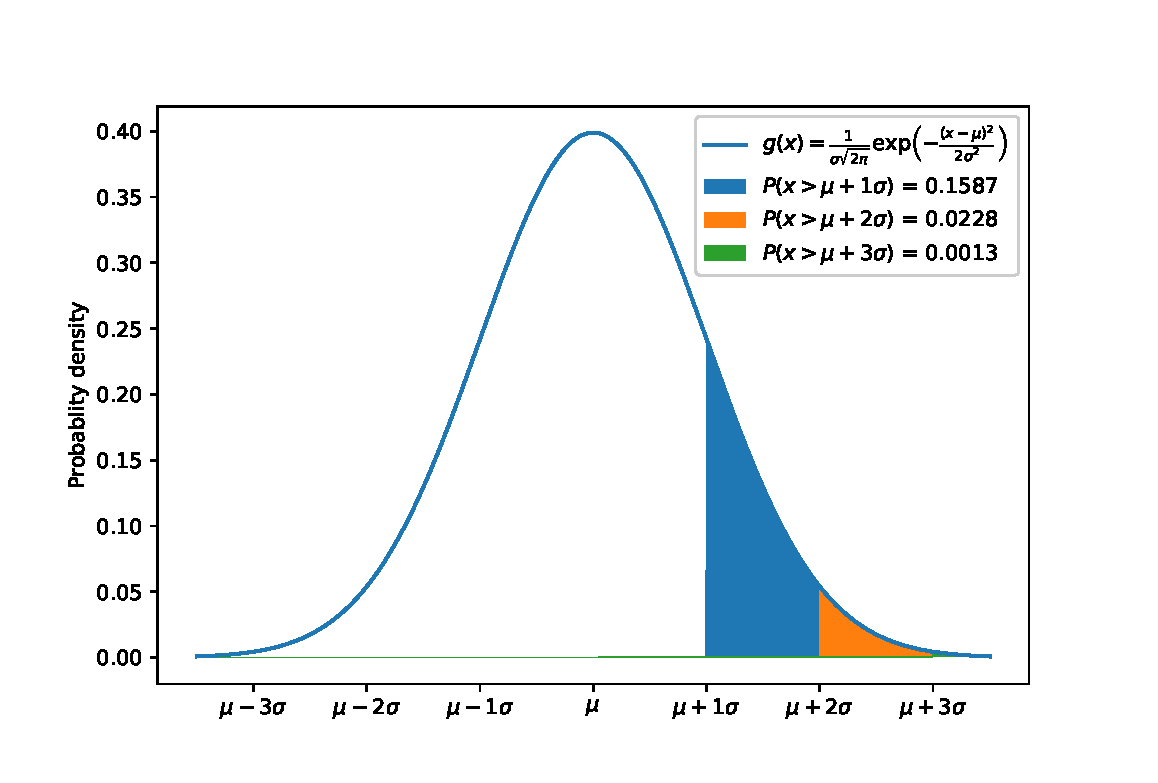
\includegraphics[width=9cm]{distribution}
\caption{Normal distribution and probability of having pixels with intensity above certain thresholds.}
\end{center}
\end{figure}

The storage space is much larger than just the pixel intensity since one needs to store as well also its position. 
Moreover, to be able to regenerate the background, the averaged and uncertainties curves needs to be stored.

The following section presents how the sparsification is performed on an example of Lysozyme (HEWL) dataset obtained using rotational data-collection.
Those data are then densified again to regenerate the data and processed in the standard XDS reduction tool \cite{xds}.
Data quality indicators are finally compared between the original dataset and the one which went through the lossy compression presented here.

\subsection{Sparsification}

The sigma-clipping algorithm was originally written for real-time sparsification of single crystal diffraction data and its integration into the LIMA2 detector control system \cite{lima} for the Jungfrau 4M detector used at ESRF ID29 is described in \cite{sri2021}.
The real-time constrain imposed to develop code running on GPU since those devices are several times
faster than equivalently priced processors.
All algorithms were developed in OpenCL \cite{opencl_khronos} and implemented in the \textit{pyFAI} software package.
A command line tool called `sparsify-Bragg' is available for off-line testing.

All the pixel coordinates and intensities are stored in a HDF5 container \cite{hdf5} following the NeXus  convention \cite{nexus}, together with a snippet of Python code explaining how to rebuild the dataset.
All sparse datasets (averaged and uncertainties curves, pixel coordinates, ...) are compressed with the bitshuffle-LZ4 \cite{bitshuffle} lossless compression.

\subsection{Densification}
Since no crystallographic software package is aware (yet) of this sparse format, the densification code was developed to regenerate initial frames and the `densify-Bragg` program was made available as part of the FabIO \cite{fabio} software package (version $\ge$0.12). 
The software constrains for this densification code are very different from the one for sparisfication since this code can be used by the final users.
For this reason `densify-Bragg' was optimized to run on multi-core CPU.
The only important options are, beside the file-format and file-name, whether the background noise has to be reconstructed or not. 
Some crystallographic reduction program like CrysAlisPro \cite{crysalis} provide a better result without noisy background while XDS \cite{xds}, which performs a deep noise analysis, needs to have the noisy background restored. 
Shaded regions are never reconstructed properly and should be masked adequately in the reduction software.

\subsection{Performances}
The performances for a lossy compression algorithm are to be evaluated along many directions: compression and decompression speeds, compression ratio and degradation of the recorded signal.
All those factors have been evaluated on a classical sample, egg white lysozyme (HEWL), and rotational data were collected on an Eiger 4M detector \cite{lysozyme}, selected for its similarity in size and performances with the Jungfrau detector. 
%This reference dataset is the one made publicly available by Dectris \cite{lysozyme} (TODO). 

\subsubsection{Compression ratio:} 
After sparsification (picking cut-off: $2\sigma$, error-model: Poisonnian), the dataset still weights 103MB which represents a 15x compression ratio compared to the standard procedure.
For conformance with the state of the art, the reference dataset was re-compressed using the bitshuffle-LZ4 algorithm \cite{bitshuffle}, for which the 1800 frames weight 1500MB (instead of the 5000GB of the original files compressed in LZ4).

The maximum theoretical compression ratio for $2\sigma$ is 22x (figure \ref{distribution}, neglecting the storage of the background data and effects of the lossless compression).
To evaluate the effective maximal compression ratio, the dataset was median-filtered along the image stack
to produce an image without peaks. 
A background dataset of 1800 such images sparsifies into a 11MB HDF5 file which represents a compression ratio of 136x ! 
Indeed, only 19 pixels were saved per frame and the compressed numerical values are mostly the same, which compresses great with bitshuffle-LZ4.

In production conditions, one would like to tune this threshold to the minimal value which guarantees a compression ratio large enough to allow the storage of all data.
For ESRF-ID29, where a Jungfrau 4M is operating at 1kHz, the pedestal+gain pre-processing convert 16-bits integers into 32-bits floating point values, doubling the bandwidth for data saving. 
The detector outputs the data via $8\times$ 10Gbit/s network links and the storage is performed via a single 25 Gbit/s link, making a minimum compression ratio of 6.4x which is equivalent to a cutoff at $1.4\sigma$ (cf. figure \ref{distribution}).


\subsubsection{Compression speed:}
%\begin{verbatim}
%kieffer@scisoft14:~/Dectris/EIGER_X_4M_lyso/demo$ sparsify-Bragg ../collect_01_00001_master.h5 -p ../geometry.poni  --bins 500 --unit="r_mm" --cycle=5 --cutoff-clip=0  --noise=1 --profile -m ../mask.npy --cutoff-pick=2.0 --error-model=poisson -o sparse.h5
%INFO:pyFAI.method_registry:Degrading method from Method(dim=1, split='pseudo', algo='histogram', impl='*', target=None) -> Method(dim=1, split='bbox', algo='histogram', impl='*', target=None)
%INFO:pyFAI.geometry:Unable to parse ../geometry.poni as JSON file, defaulting to PoniParser
%WARNING:pyFAI.ext.splitBBoxCSR:Pixel splitting desactivated !
%INFO:silx.opencl.processing:379.313MB are needed on device: TITAN V,  which has 12652.839MB
%INFO:silx.opencl.processing:Compiling file ['silx:opencl/doubleword.cl', 'pyfai:openCL/preprocess.cl', 'pyfai:openCL/memset.cl', 'pyfai:openCL/ocl_azim_CSR.cl', 'pyfai:openCL/peak_finder.cl', 'pyfai:openCL/peakfinder8.cl'] with options -D NBINS=500  -D NIMAGE=4485690 -D WORKGROUP_SIZE=1024
%INFO:silx.opencl.processing:■■■■■■■■■■■■■■■■■■■]  100%  Saving: sparse.h5                      
%OpenCL kernel profiling statistics in milliseconds for: OCL_PeakFinder
%                                       Kernel name (count):      min   median      max     mean      std
%                                 copy H->D indices (    1):    3.730    3.730    3.730    3.730    0.000
%                                  copy H->D indptr (    1):    0.001    0.001    0.001    0.001    0.000
%                                    copy H->D mask (    1):    1.096    1.096    1.096    1.096    0.000
%                                copy H->D radius1d (    1):    0.002    0.002    0.002    0.002    0.000
%                                copy H->D radius2d (    1):    3.489    3.489    3.489    3.489    0.000
%                               copy raw H->D image ( 1800):    3.615    5.064    5.718    4.893    0.412
%                                 cast u32_to_float ( 1800):    0.070    0.075    0.103    0.074    0.001
%                                         memset_ng ( 1800):    0.004    0.004    0.010    0.004    0.000
%                                       corrections ( 1800):    0.169    0.171    0.178    0.172    0.001
%                                   csr_sigma_clip4 ( 1800):    3.077    3.230    4.140    3.267    0.133
%                                    memset counter ( 1800):    0.004    0.004    0.015    0.004    0.001
%                                       peak_search ( 1800):    0.261    0.263    0.272    0.263    0.001
%                                 copy D->H counter ( 1800):    0.001    0.001    0.010    0.001    0.000
%                  copy D->D + cast uint32 intenity ( 1800):    0.007    0.010    0.025    0.010    0.002
%                           copy D->H peak_position ( 1800):    0.003    0.006    0.029    0.009    0.005
%                           copy D->H peak_intensty ( 1800):    0.003    0.006    0.029    0.009    0.005
%                          copy D->H background_avg ( 1800):    0.002    0.002    0.004    0.002    0.000
%                          copy D->H background_std ( 1800):    0.002    0.002    0.003    0.002    0.000
%________________________________________________________________________________
%                       Total OpenCL execution time        : 15687.401ms
%\end{verbatim}

The compression speed has been measured on the computer designed for online data-reduction of the Jungfrau detector \cite{sri2021}: 
an IBM AC922 using two Power9 processors and two (up to four) Nvidia Tesla V100 GPU. 
The sequential execution of the code on the GPU takes about 4 ms to process one image and uses one single CPU-core and a quarter of a GPU. 
In online condition, multiple parallel processes are expected to achieve much higher frame-rate, since the nominal speed for the Jungfrau is 1kHz.

\subsubsection{Decompression speed:} 
The decompression of those data should typically be performed on a standard workstation (here running two Intel Xeon Gold 6134 CPU @ 3.20GHz): the reconstruction speed is found to take 30 s while the writing of the densified dataset (with bitshuffle-LZ4 compression) takes 45s. 
%maybe explicit that the decompression is for the full dataset and not 30s per frame
Densification is thus faster than writing on disk.
The reading of the input sparse dataset is negligible (<2s).

\subsubsection{Quality of the restored dataset:} 
The densified dataset was processed via XDS and the summary indicator for the quality of the results are compared with the one coming from the reduction of the original dataset. 
Since those integrator are measured on integral peaks with $I/\sigma>3$ and the sparsification was performed
with a cut-off of 2, those result should be almost unaffected, which is confirmed in the table \ref{xds_summary}.

\begin{table}
\label{xds_summary}
\caption{Quality indicators after peak integration and averaging using XDS \cite{xds}. 
Lysozyme (HEWL) dataset provided by Dectris for advertising their Eiger-4M detector \cite{lysozyme}.}.
\begin{tabular}{|c|c c c|c c c|} 
\hline
Indicator & \multicolumn{3}{c|}{Initial dataset} & \multicolumn{3}{c|}{Lossy compressed dataset ($2\sigma$)} \\ 
          & 2.91\AA & 2.06\AA & all & 2.91\AA & 2.06\AA & all \\
\hline
Completeness                                        & 98.8& 90.8 & 93.8\% & 99.8& 90.6 & 93.5\% \\ 
$R_{obs}=\frac{\sum |I_{h,i}-I_{i}|}{\sum I_{h,i}}$ & 9.9 & 57.3& 12.5\% & 9.2 & 61.2&  11.4\%\\ 
$R_{expected}$                                      & 8.8 & 73.2& 15.0\% & 8.2 & 68.7 &  12.1\%\\
$R_{meas}$ \cite{Rmeas}  &10.3 &61.2& 13.2\% & 9.6 & 65.5 & 12.0\%\\
$CC_{1/2}$ \cite{cc1/2}  & 99.7 &94.0 & 99.7   & 99.6 & 95.4 & 99.7  \\
$<I/\sigma>$               & 25.80 & 5.39 & 10.52  & 26.33& 4.09 & 10.17 \\
\hline
\end{tabular}
\end{table}


\section{Application to serial crystallography}
A classical way of pre-processing serial-crystallography data is to shrink the amount of data by sieving-out empty or bad frames, actually keeping frame which deserve processing. 
This is the role of the "veto-algorithms".

The sigma clipping algorithm provides us with the background (average and deviation) and is used to pick pixels which are likely to be peaks. 
For this,  several additional checks are performed on the local neighborhood which is a small square patch (typically 3x3 or 5x5 pixels):
\begin{itemize}
\item The considered pixel is the maximum of the local neighborhood.
\item Enough of pixels in the local neighborhood satisfying the SNR condition: typically 2 to 5 pixels out of 9 or 25 are intense enough.
\end{itemize}

For each peak, the pixel coordinate, the precise centroïd, the sum of data and its propagated deviation are recorded and reported. 
Those peak-position are saved into a HDF5 file (represented figure \ref{silx}) following the CXI format \cite{cxi} which can be can be read from CrystFEL \cite{CrystFEL}.
CrystFEL is the swiss-knife of serial-crystallography which allows to swap peak-picking algorithms \cite{zaefferer, Cheetah2014, robustpeakfinder} and indexing tools \cite{xds, mosflm, taketwo, xgandalf, pinkindexer}.
Since indexing is compute intensive, CrystFEL can distributes calculation over several cores or nodes.

\begin{figure}
\label{silx}
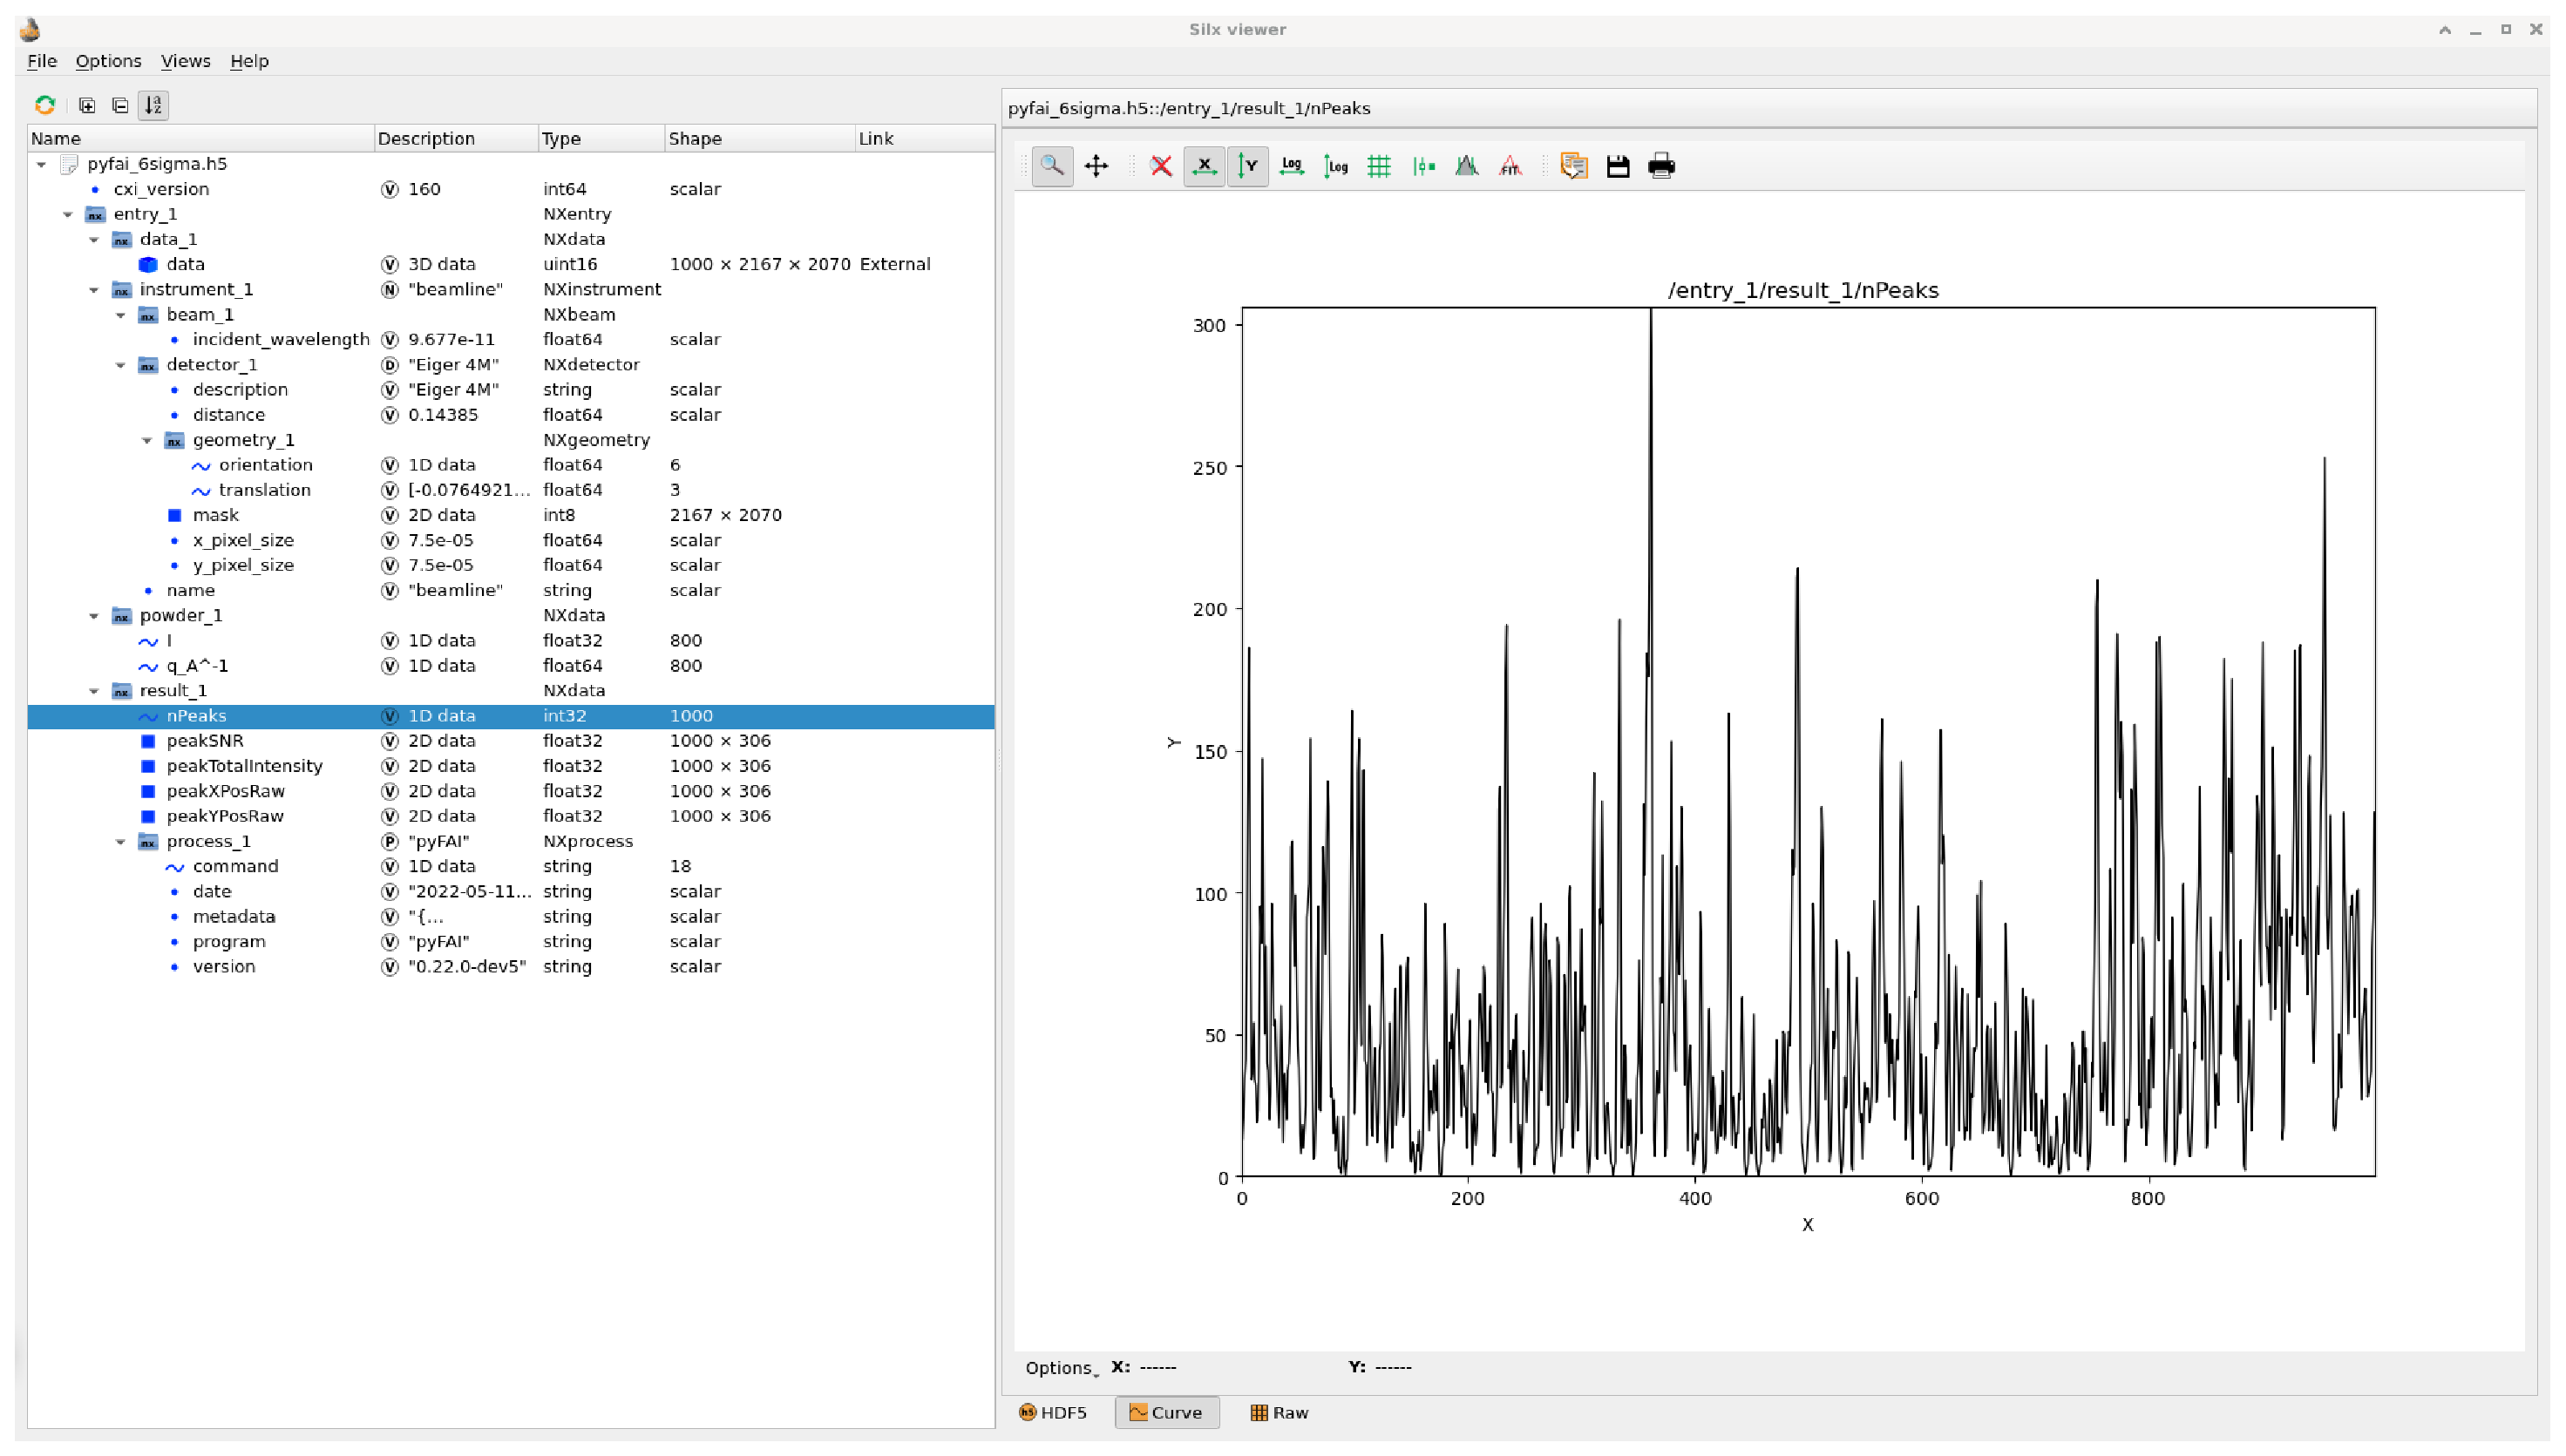
\includegraphics[width=12cm]{silx_view}
\caption{Peak-picking CXI-file produced by pyFAI and visualized with the \textit{silx viewer} \cite{silx}.
The left-hand side contains the HDF5 tree structure while the right-hand side presents the default plot with the number of peaks found per frame.}
\end{figure}


The serial crystallography beam-line will use NanoPeakCell \cite{nanopeakcell} for online visualization and feed-back to check if peaks found correspond actually the crystal lattice of the sample.

We will first compare the peak-picking algorithm with some reference implementation on a single frame before
evaluating the quality of the picked points on a serial-crystallography dataset where the indexation rate will be used as quality indicator for the picking.

\subsection{Comparison of picked peaks}
Figure \ref{peakfinder} presents the comparison between the original \textit{peakfinder8} described in \citeasnoun{Cheetah2014}, interfaced in Python via OnDA \cite{onda} and the version implemented into pyFAI on the same Pilatus 6M image, already used in figure \ref{fig1}. 

\begin{figure}
\label{peakfinder}
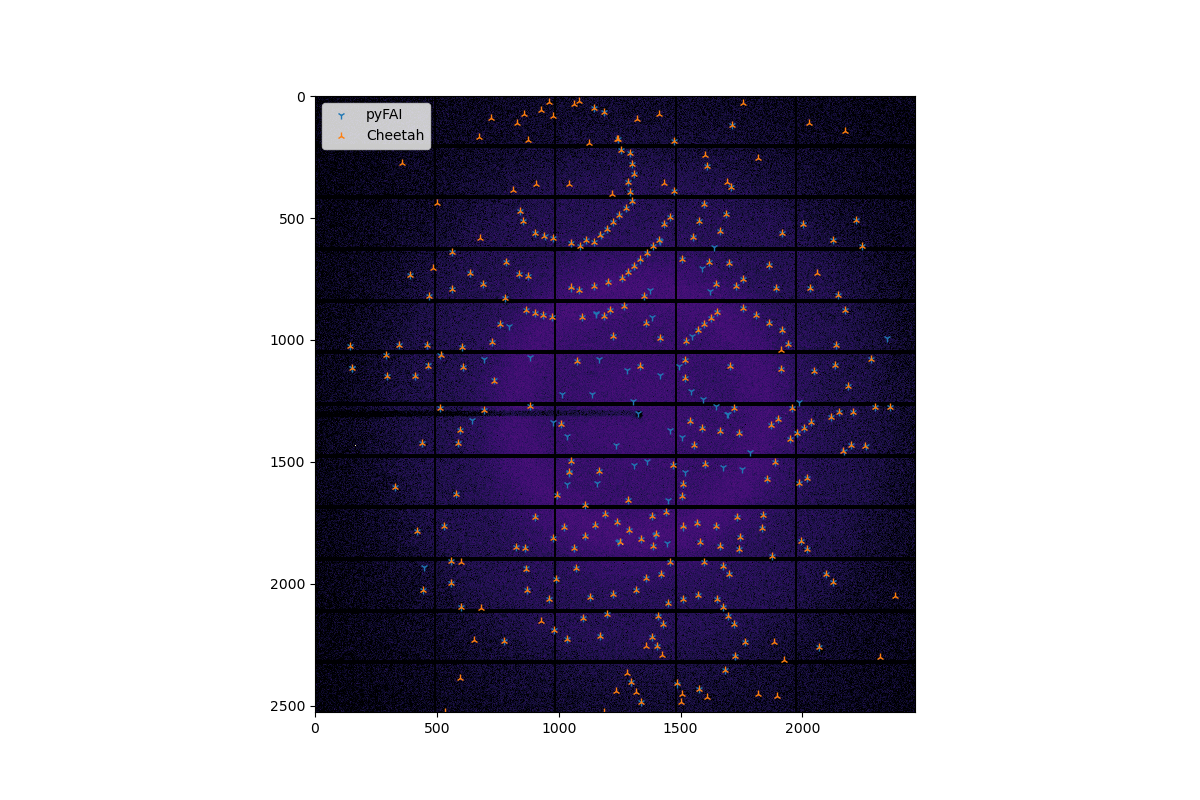
\includegraphics[width=12cm]{peakfinder}
\caption{Comparison of the reference \textit{peakfinder8} interfaced with Onda (in orange, execution time 300ms) and the version from pyFAI (in light blue, execution time 10ms) on top of a Pilatus 6M diffraction frame (insulin).}
\end{figure}

In figure \ref{peakfinder}, most peak found by both implementation match and superimpose with Bragg-peaks.
There are more blue-peaks (found by pyFAI) closer to the beam center while more orange peaks (found by Onda) are located in the outer-shell.
This plot was made with a minimum SNR of three and a noise level of one since the Pilatus detector is Poissonian.
Peaks were registered if four pixels meet the SNR criterion in a 5x5 pixels patch around the peak.
Those parameters have been tuned to obtain a comparable number of peaks with both implementations: 290 with pyFAI and 293 with Onda.
The similarity of those figures allows a direct comparison of peaks found per resolution shell, histogram plotted in figure \ref{peak_per_ring}.

\begin{figure}
\label{peak_per_ring}
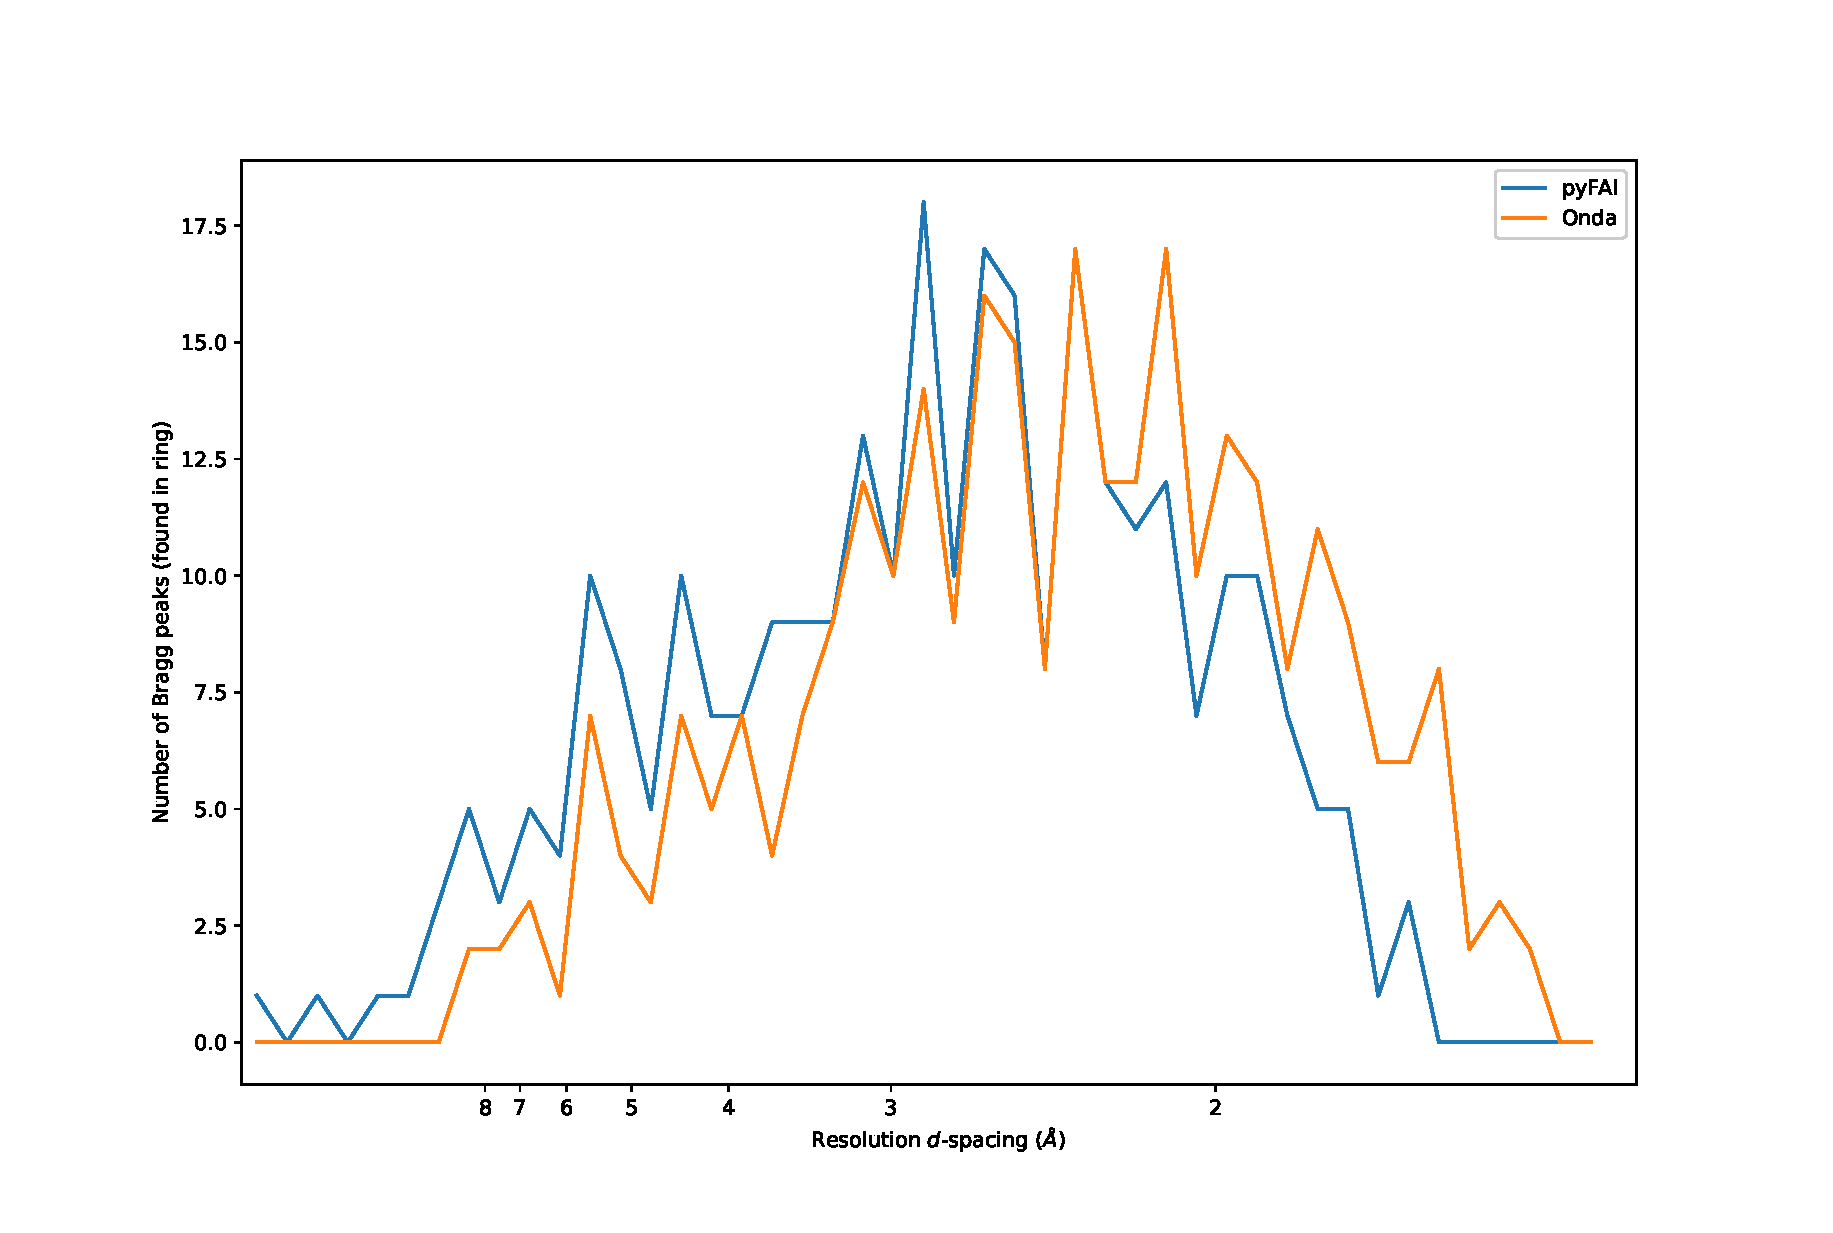
\includegraphics[width=12cm]{peak_per_ring}
\caption{Number of peaks found in the different resolution shell for the \textit{peakfinder} implemented in pyFAI and in Onda. The width of each of the shell is one inverse nanometer.}
\end{figure}

The analysis of the histogram in figure \ref{peak_per_ring} confirms the implementation in pyFAI is getting more points closer to the beam-center while the reference implementation is picking more point at larger q-values.
This is likely due to the curvature of the Debye-Scherrer ring: the original version of peakfinder8 evaluates the variance in a neighborhood defined by some radius around the point of interest and the variance is higher close to the beam-center due to the important curvature of those rings.
On the opposite, pyFAI knows about this curvature and measures the variance along the ring.
Points picked by Onda at larger q-values do not look like Bragg-peaks but this could be a side-effect of the parameter tuning to get the same number of peaks for both algorithms.

A word on performances: the Python binding in Onda to the peakfinder8 algorithm from Cheetah runs in 180ms on a high-end server CPU (AMD Epyc 7262) and 300ms on a workstation (Intel Xeon E5-1650 v4). 
The version available in pyFAI was designed in OpenCL \cite{opencl_khronos, opencl, pyopencl} and runs best on GPUs: 30ms on a AMD Vega 56 and in 10 ms on a Nvidia RTX A5000. 
Interestingly, an entry level GPU (Nvidia GT1030), which is seven times cheaper than the Epyc processor, shows the same performances (but this CPU has eight cores).

\subsection{Quality of the peakfinder on serial crystallography data}

The quality of peaks extracted with this algorithm is finally evaluated on a serial-crystallography dataset: tiny crystals of egg white lysozyme (HEWL) were deposited on a SiN membrane and this membrane was scanned in front of the beam at the ID30B beamline at the ESRF with an Eiger-4M detector.
A fraction of 1000 frames of the dataset \cite{ssx-Lyso} was used as a probe and was indexed with the \textit{indexamajig} tool from CrystFEL. 
Since all frames show Bragg-peaks (figure \ref{silx}) the number of indexed frames can be seen as a quality indicator of the peak-picking algorithm used, when all other parameter remain unchanged.
The indexation was performed with the \textsc{xgandalf} algorithm \cite{xgandalf} with default settings from CrystFEL 0.10.1 and was provided with the cell parameter: tetragonal $a=b=78.77\text{\AA}; c=39.04\text{\AA}; \alpha=\beta=\gamma = 90^o$.
The table \ref{crystfel} compares the number of frames properly indexed with the different picking algorithms available in CrystFEL and with the algorithm presented here. 

\begin{table}
\label{crystfel}
\caption{Indexation rate obtained with \textsc{xgandalf} \cite{xgandalf} from peak positions extracted with different picking algorithms available from CrystFEL \cite{CrystFEL} on a subset of 1000 frames of microcrystals of Lysozyme (HEWL) collected with an Eiger 4M at ESRF ID30b.}
\begin{center}
\begin{tabular}{|c|c|c|c|c|} 
\hline
Peak-picking  & \multicolumn{2}{c|}{\textsc{xgandalf} (default)} & \multicolumn{2}{c|}{\textsc{xgandalf} (fast)}\\
method & Index. rate & run-time & Index. rate & run-time \\ 
\hline
Zaef \cite{zaefferer} & 100\textperthousand & 2178 s & 100\textperthousand& 430 s\\
PeakFinder8 \cite{Cheetah2014} & 495\textperthousand& 10397 s &485\textperthousand & 1757 s\\
PeakFinder9 \cite{CrystFEL} & 442\textperthousand& 8328 s&435\textperthousand&1436 s\\
RobustPF \cite{robustpeakfinder} & 224\textperthousand& 6314 s& 212\textperthousand& 1628 s \\
pyFAI (this contribution) & 497\textperthousand& 9325 s& 492\textperthousand &1595 s\\
\hline
\end{tabular}
\end{center}
\end{table}

Since the Eiger detector is a counting detector, the global threshold for algorithms \textit{zaef} and \textit{peakfinder8} had to be lowered (to 50, which is the maximum of the background signal on any frame) and the the default SNR value was used for \textit{zaef}, \textit{peakfinder8}. 
The same SNR value of five was used for \textit{pyFAI}.
Default parameters were used for \textit{PeakFinder9} and \textit{RobustPeakFinder} algorithms.
The reported run-time correspond to the execution time on a single core of an Intel Xeon Gold 6134.


The indexing rate obtained with the algorithm from pyFAI is in par with reference implementations like \textit{peakfinder8} or \textit{peakfinder9} available from CrystFEL. 
Since time is mostly spent in indexing, sets of peaks which are simpler to index present lower run-time since fewer retry were needed. 
Table \ref{crystfel} presents also the indexing performances when using the option \textit{--xgandalf-fast-execution} from \textit{indexamajig}, which is five to six times faster and exhibits a limited degradation of the indexing rate.
The peak extraction in pyFAI is about as fast as the sparsification, so it can be used online to perform the pre-analysis and provide peaks to NanoPeakCell. 
Nevertheless the executable `peakfinder` available from pyFAI (offline tool) has a total execution time which is much larger: about 30 s for 1000 frames, most of which is spent in reading and writing the different HDF5 files.

\section{Conclusion}

Background analysis of single crystal diffraction images can be implemented efficiently using iterative azimuthal integration and allows the separation of the signal originating from Bragg-peaks from amorphous background.

A first application presented is lossy compression of diffraction frames where the average background is saved on the one side and the position and the intensity of pixels belonging to peaks on the the other.
The quality of the compression has been demonstrated on rotational macro-molecular crystallography where the degradation of the signal has been monitored after a cycle of compression-decompression and the analysis of those dataset with standard reduction tools (XDS).

The second application is a peak-finder for synchrotron serial crystallography which locates peak positions in real time and can be used to discard frames. 
The quality of the picking has been evaluated by comparing the indexation rate with reference peak-finder algorithms.

     %-------------------------------------------------------------------------
     % The back matter of the paper - acknowledgements and references
     %-------------------------------------------------------------------------

     % Acknowledgements come after the appendices

\ack{Acknowledgements}
The authors would like to thank Gavin Vaughan, scientist at Materials beamline at the ESRF,  for the constructive discussion about sigma-clipping versus median filtering. 
We would like to thank also Jonathan P. Wright and Carlotta Giacobbe for offering us the ability to test those algorithms on small molecule data and validate the concept on the ID11 beamline at the ESRF.


\bibliographystyle{iucr}
\bibliography{biblio}

\end{document}                    % DO NOT DELETE THIS LINE
%%%%%%%%%%%%%%%%%%%%%%%%%%%%%%%%%%%%%%%%%%%%%%%%%%%%%%%%%%%%%%%%%%%%%%%%%%%%%%
